\documentclass[tikz,border=14pt]{standalone}
\usepackage{tikz}
\usetikzlibrary{positioning, fit, arrows.meta, backgrounds, calc, shadows}

\begin{document}
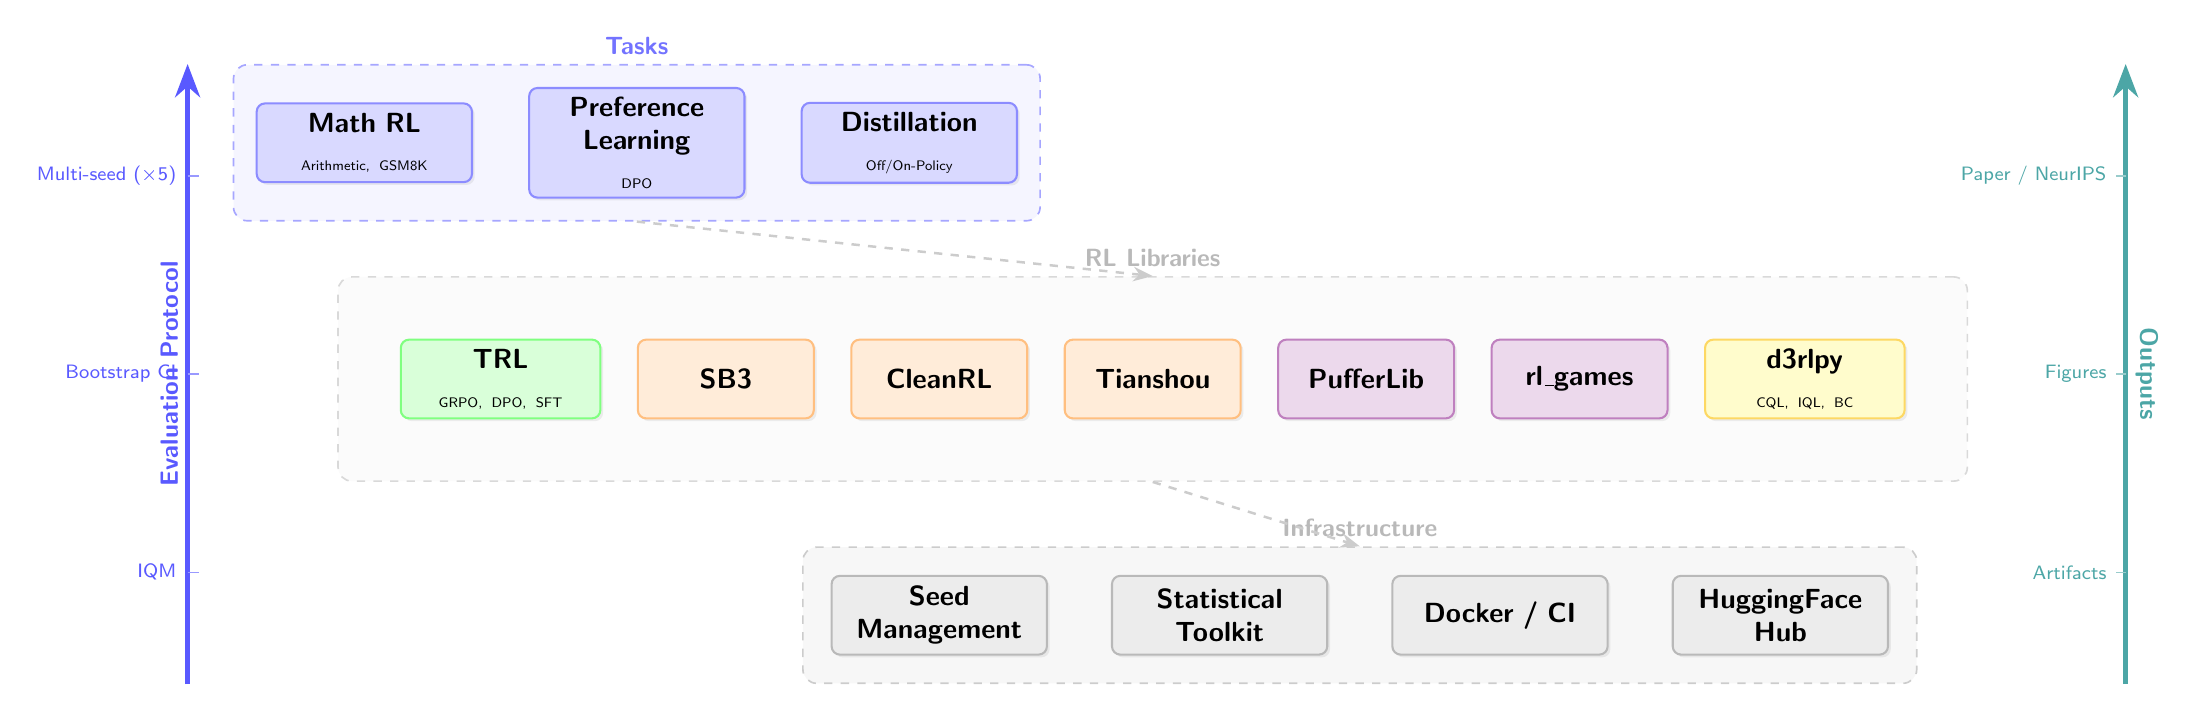
\begin{tikzpicture}[
  font=\sffamily,
  base/.style={
    draw, rounded corners=3pt, align=center,
    minimum height=1.0cm, text width=2.5cm,
    line width=0.75pt,
    drop shadow={shadow xshift=1pt, shadow yshift=-1pt, opacity=0.13}
  },
  task/.style={base, fill=blue!15, draw=blue!45},
  llmnative/.style={base, fill=green!15, draw=green!50, text width=2.3cm},
  classicrl/.style={base, fill=orange!15, draw=orange!50, text width=2.0cm},
  highperf/.style={base, fill=violet!15, draw=violet!50, text width=2.0cm},
  offline/.style={base, fill=yellow!20, draw=yellow!55!orange!60, text width=2.3cm},
  infra/.style={base, fill=gray!15, draw=gray!55, text width=2.5cm},
  groupbox/.style={draw, dashed, rounded corners=5pt, inner sep=8pt, line width=0.6pt},
  sidebar/.style={line width=2pt, -Stealth},
]

%% ─────────────────────────────────────────────────────
%% LAYER 1: Tasks
%% ─────────────────────────────────────────────────────
\node[task] (math)   at (0,0) {\textbf{Math RL}\\[2pt]{\tiny Arithmetic, GSM8K}};
\node[task] (pref)   [right=0.7cm of math]
  {\textbf{Preference}\\[0pt]\textbf{Learning}\\[2pt]{\tiny DPO}};
\node[task] (distil) [right=0.7cm of pref]
  {\textbf{Distillation}\\[2pt]{\tiny Off/On-Policy}};

\begin{scope}[on background layer]
  \node[groupbox, fill=blue!4, draw=blue!35,
        label={[font=\sffamily\bfseries\small, text=blue!55]above:Tasks}]
    (taskgrp) [fit=(math)(pref)(distil)] {};
\end{scope}

%% ─────────────────────────────────────────────────────
%% LAYER 2: RL Libraries
%% ─────────────────────────────────────────────────────
\node[llmnative] (trl) at ([yshift=-3.0cm]$(math)!0.5!(pref)$)
  {\textbf{TRL}\\[2pt]{\tiny GRPO, DPO, SFT}};
\node[classicrl] (sb3)       [right=0.45cm of trl]    {\textbf{SB3}};
\node[classicrl] (cleanrl)   [right=0.45cm of sb3]    {\textbf{CleanRL}};
\node[classicrl] (tianshou)  [right=0.45cm of cleanrl]{\textbf{Tianshou}};
\node[highperf]  (pufferlib) [right=0.45cm of tianshou]{\textbf{PufferLib}};
\node[highperf]  (rlgames)   [right=0.45cm of pufferlib]{\textbf{rl\_games}};
\node[offline]   (d3rlpy)    [right=0.45cm of rlgames]
  {\textbf{d3rlpy}\\[2pt]{\tiny CQL, IQL, BC}};

\begin{scope}[on background layer]
  \node[groupbox, fill=green!4, draw=green!40,
        label={[font=\sffamily\tiny\bfseries, text=green!60!black]below:LLM-native}]
    (llmgrp) [fit=(trl)] {};
  \node[groupbox, fill=orange!4, draw=orange!35,
        label={[font=\sffamily\tiny\bfseries, text=orange!70!black]below:Classic RL}]
    (classicgrp) [fit=(sb3)(cleanrl)(tianshou)] {};
  \node[groupbox, fill=violet!4, draw=violet!35,
        label={[font=\sffamily\tiny\bfseries, text=violet!70!black]below:High-Perf}]
    (highperfgrp) [fit=(pufferlib)(rlgames)] {};
  \node[groupbox, fill=yellow!4, draw=yellow!50!orange!40,
        label={[font=\sffamily\tiny\bfseries, text=yellow!60!black]below:Offline}]
    (offlinegrp) [fit=(d3rlpy)] {};
  \node[groupbox, fill=gray!3, draw=gray!30, inner sep=14pt,
        label={[font=\sffamily\bfseries\small, text=gray!55]above:RL Libraries}]
    (libgrp) [fit=(llmgrp)(classicgrp)(highperfgrp)(offlinegrp)] {};
\end{scope}

%% ─────────────────────────────────────────────────────
%% LAYER 3: Infrastructure
%% ─────────────────────────────────────────────────────
\node[infra] (seedmgmt) at ([yshift=-3.0cm]$(sb3)!0.5!(tianshou)$)
  {\textbf{Seed}\\[0pt]\textbf{Management}};
\node[infra] (statstk)  [right=0.8cm of seedmgmt] {\textbf{Statistical Toolkit}};
\node[infra] (docker)   [right=0.8cm of statstk]  {\textbf{Docker / CI}};
\node[infra] (hf)       [right=0.8cm of docker]   {\textbf{HuggingFace Hub}};

\begin{scope}[on background layer]
  \node[groupbox, fill=gray!6, draw=gray!40, inner sep=10pt,
        label={[font=\sffamily\bfseries\small, text=gray!55]above:Infrastructure}]
    (infragrp) [fit=(seedmgmt)(statstk)(docker)(hf)] {};
\end{scope}

%% ─────────────────────────────────────────────────────
%% Layer connectors
%% ─────────────────────────────────────────────────────
\begin{scope}[on background layer]
  \draw[-Stealth, gray!40, line width=0.9pt, dashed]
    (taskgrp.south) -- (libgrp.north);
  \draw[-Stealth, gray!40, line width=0.9pt, dashed]
    (libgrp.south)  -- (infragrp.north);
\end{scope}

%% ─────────────────────────────────────────────────────
%% LEFT SIDE — Evaluation Protocol
%% Anchored 2cm left of libgrp (widest layer)
%% ─────────────────────────────────────────────────────
\coordinate (EvalX)      at ([xshift=-1.9cm]libgrp.west);
\coordinate (evaltop)    at (EvalX |- taskgrp.north);
\coordinate (evalbottom) at (EvalX |- infragrp.south);

\draw[sidebar, color=blue!65] (evalbottom) -- (evaltop);

\node[rotate=90, anchor=south, font=\sffamily\bfseries\small, text=blue!65]
  at ($(evaltop)!0.5!(evalbottom)$) {Evaluation Protocol};

\foreach \frac/\lbl in {0.18/Multi-seed (\texttimes5), 0.50/Bootstrap CI, 0.82/IQM}{
  \draw[blue!40, line width=0.7pt]
    ($(evaltop)!\frac!(evalbottom)$) -- ++(0.15cm,0);
  \node[anchor=east, font=\sffamily\scriptsize, text=blue!65, xshift=-0.02cm]
    at ($(evaltop)!\frac!(evalbottom)$) {\lbl};
}

%% ─────────────────────────────────────────────────────
%% RIGHT SIDE — Outputs
%% Anchored 2.8cm right of libgrp; labels inside the gap
%% ─────────────────────────────────────────────────────
\coordinate (OutX)      at ([xshift=2.0cm]libgrp.east);
\coordinate (outtop)    at (OutX |- taskgrp.north);
\coordinate (outbottom) at (OutX |- infragrp.south);

\draw[sidebar, color=teal!70] (outbottom) -- (outtop);

%% "Outputs" label rotated on the arrow, with three sub-labels also rotated
\node[rotate=-90, anchor=south, font=\sffamily\bfseries\small, text=teal!70]
  at ($(outtop)!0.5!(outbottom)$) {Outputs};

%% Labels between libgrp.east and the Outputs arrow (anchor=east toward arrow)
\node[anchor=east, font=\sffamily\scriptsize, text=teal!70, xshift=-0.12cm]
  at ($(outtop)!0.18!(outbottom)$) {Paper / NeurIPS};

\node[anchor=east, font=\sffamily\scriptsize, text=teal!70, xshift=-0.12cm]
  at ($(outtop)!0.50!(outbottom)$) {Figures};

\node[anchor=east, font=\sffamily\scriptsize, text=teal!70, xshift=-0.12cm]
  at ($(outtop)!0.82!(outbottom)$) {Artifacts};

\foreach \frac in {0.18,0.50,0.82}{
  \draw[teal!40, line width=0.7pt]
    ([xshift=-0.12cm]$(outtop)!\frac!(outbottom)$) -- ++(0.12cm,0);
}

\end{tikzpicture}
\end{document}
